\documentclass{beamer}
\usepackage{graphicx}
\usepackage{amsmath}
\usetheme{Warsaw}
\title{PDP Homework\#2: Matrix multiplication in MPI}
\author{Wen-Chieh Wu}
\date{March 26, 2014}
\begin{document}
\maketitle
\begin{frame}
\frametitle{Matrix multiplication}
\begin{center}
  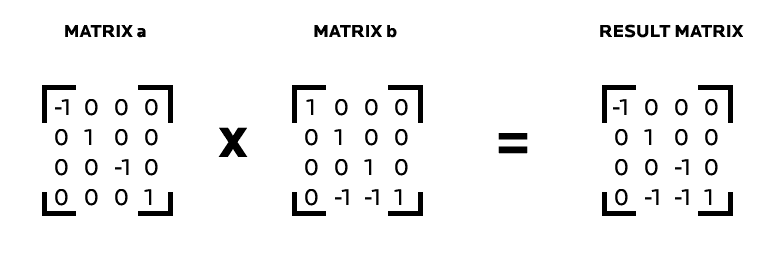
\includegraphics[scale=0.35]{img/img01.png}
\end{center}
\end{frame}

\begin{frame}
  \frametitle{Input \& Output}
  \begin{exampleblock}{Input}
    Given n matrices which are NxN
  \end{exampleblock}
  
  \begin{exampleblock}{Output}
    Output the summation of all elements in each self-multiplied matrices, each line output 1 result, there will be n lines.
  \end{exampleblock}
\end{frame}

\begin{frame}
\frametitle{Example}
Given
$$
\begin{bmatrix}
  -1 & 2\\
  2 & 3
\end{bmatrix}
$$
You need to calculate
$$
\begin{bmatrix}
  -1 & 2\\
  2 & 3
\end{bmatrix}
\begin{bmatrix}
  -1 & 2\\
  2 & 3
\end{bmatrix}
=
\begin{bmatrix}
  5 & 4\\
  4 & 13
\end{bmatrix}
$$
And find the summation of all elements
$$
5+4+4+13=26
$$
\end{frame}

\begin{frame}
  \frametitle{Goal}
  \begin{center}
    {\huge Write a MPI version of matrices multiplication}
  \end{center}
\end{frame}

\begin{frame}
  \frametitle{Example program}
  Obtain and execute the example program
  \begin{itemize}
    {\item \$ cp -r /tmp/mpi.example .}
    {\item \$ cd mpi.example}
    {\item \$ gcc mat.c -o mat -lm}
    {\item \$ ./mat input11.dat 1 1}
  \end{itemize}
  Input data representation
  \begin{itemize}
    {\item input11.dat}: 10 10x10 matrices
    {\item input22.dat}: 100 100x100 matrices
    {\item input32.dat}: 1000 100x100 matrices
    {\item input42.dat}: 10000 100x100 matrices
  \end{itemize}
\end{frame}

\begin{frame}
  \frametitle{Environment}
  There are 6 machines with 12 cores, totally there are {\bf 72} cores
  \begin{itemize}
    {\item h92}
    {\item data01}
    {\item data02}
    {\item data03}
    {\item data04}
    {\item data05}
  \end{itemize}
  You can use all of them at the same time by using {\bf hosts} in mpi.example\\
  \$ mpirun -n 72 -hostfile hosts [program] [input\_data] [var1] [var2]
\end{frame}

\begin{frame}
  \frametitle{Submit}
  \begin{itemize}
    {\item Files you need to upload}
      \begin{itemize}
        {\item mat.mpi.c}
        {\item readme.txt}
      \end{itemize}
    {\item You should zip these two files and upload to CEIBA, ex. r01922003.zip}
    {\item In readme.txt, please decribe how to run your program, including how many processes you use}\\
      EX. mpirun -n 10 ./mat.mpi input11.dat 1 1
  \end{itemize}
\end{frame}

\begin{frame}
  \frametitle{Grading}
  \begin{itemize}
    {\item If you pass 4 test data in time, you will get 80 points.}
    {\item The rest 20 points will be given by another ``huge'' test data.}
    {\item Each week late will take 10\% of the final grade.}
  \end{itemize}
\end{frame}

\begin{frame}
  \frametitle{Note}
  \begin{itemize}
    {\item Feel free to ask questions on CEIBA, this homework is much harder than the first one.}
    {\item If you have any question, e-mail to r01922003@ntu.edu.tw.}
  \end{itemize}
\end{frame}

\end{document}
